\documentclass[../main/NEMO_manual]{subfiles}

\begin{document}

\chapter{Configurations}
\label{chap:CFGS}

\chaptertoc

\paragraph{Changes record} ~\\

{\footnotesize
  \begin{tabularx}{\textwidth}{l||X|X}
    Release & Author(s) & Modifications \\
    \hline
    {\em   4.0} & {\em ...} & {\em ...} \\
    {\em   3.6} & {\em ...} & {\em ...} \\
    {\em   3.4} & {\em ...} & {\em ...} \\
    {\em <=3.4} & {\em ...} & {\em ...}
  \end{tabularx}
}

\clearpage

%% =================================================================================================
\section{Introduction}
\label{sec:CFGS_intro}

The purpose of this part of the manual is to introduce the \NEMO\ reference configurations.
These configurations are offered as means to explore various numerical and physical options,
thus allowing the user to verify that the code is performing in a manner consistent with that we are running.
This form of verification is critical as one adopts the code for his or her particular research purposes.
The reference configurations also provide a sense for some of the options available in the code,
though by no means are all options exercised in the reference configurations.
Configuration is defined manually through the \nam{cfg}{cfg} namelist variables.

\begin{listing}
  \nlst{namcfg}
  \caption{\forcode{&namcfg}}
  \label{lst:namcfg}
\end{listing}

%% =================================================================================================
\section[C1D: 1D Water column model (\texttt{\textbf{key\_c1d}})]{C1D: 1D Water column model (\protect\key{c1d})}
\label{sec:CFGS_c1d}

The 1D model option simulates a stand alone water column within the 3D \NEMO\ system.
It can be applied to the ocean alone or to the ocean-ice system and can include passive tracers or a biogeochemical model.
It is set up by defining the position of the 1D water column in the grid
(see \path{./cfgs/SHARED/namelist\_ref}).
The 1D model is a very useful tool
\textit{(a)} to learn about the physics and numerical treatment of vertical mixing processes;
\textit{(b)} to investigate suitable parameterisations of unresolved turbulence
(surface wave breaking, Langmuir circulation, ...);
\textit{(c)} to compare the behaviour of different vertical mixing schemes;
\textit{(d)} to perform sensitivity studies on the vertical diffusion at a particular point of an ocean domain;
\textit{(d)} to produce extra diagnostics, without the large memory requirement of the full 3D model.

The methodology is based on the configuration of the smallest possible domain:
a 3x3 domain with 75 vertical levels.

The 1D model has some specifies. First, all the horizontal derivatives are assumed to be zero,
and second, the two components of the velocity are moved on a $T$-point.
Therefore, defining \key{c1d} changes some things in the code behaviour:
\begin{enumerate}
\item a simplified \rou{stp} routine is used (\rou{stp\_c1d}, see \mdl{step\_c1d} module) in which
  both lateral tendancy terms and lateral physics are not called;
\item the vertical velocity is zero
  (so far, no attempt at introducing a Ekman pumping velocity has been made);
\item a simplified treatment of the Coriolis term is performed as $U$- and $V$-points are the same
  (see \mdl{dyncor\_c1d}).
\end{enumerate}
All the relevant \textit{\_c1d} modules can be found in the src/OCE/C1D directory of
the \NEMO\ distribution.

% to be added:  a test case on the yearlong Ocean Weather Station (OWS) Papa dataset of Martin (1985)

%% =================================================================================================
\section{ORCA family: global ocean with tripolar grid}
\label{sec:CFGS_orca}

The ORCA family is a series of global ocean configurations that are run together with
the SI3 model (ORCA-ICE) and possibly with PISCES biogeochemical model (ORCA-ICE-PISCES).
An appropriate namelist is available in \path{./cfgs/ORCA2_ICE_PISCES/EXPREF/namelist_cfg} for ORCA2.
The domain of ORCA2 configuration is defined in \textit{ORCA\_R2\_zps\_domcfg.nc} file,
this file is available in tar file on the \NEMO\ community zenodo platform: \\
https://doi.org/10.5281/zenodo.2640723

In this namelist\_cfg the name of domain input file is set in \nam{cfg}{cfg} block of namelist.

\begin{figure}[!t]
  \centering
  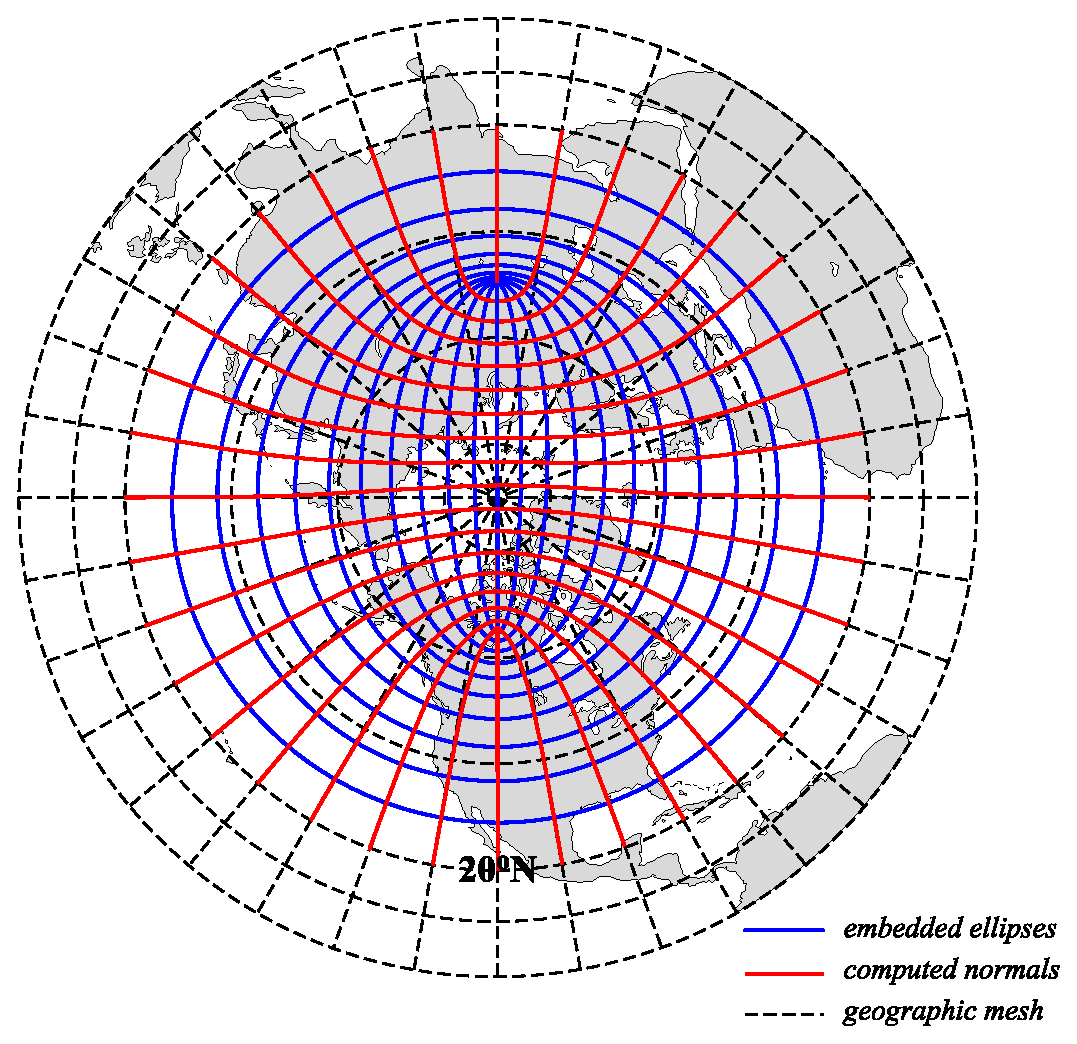
\includegraphics[width=0.66\textwidth]{CFGS_ORCA_NH_mesh}
  \caption[ORCA mesh conception]{
    ORCA mesh conception.
    The departure from an isotropic Mercator grid start poleward of 20\deg{N}.
    The two "north pole" are the foci of a series of embedded ellipses (blue curves) which
    are determined analytically and form the i-lines of the ORCA mesh (pseudo latitudes).
    Then, following \citet{madec.imbard_CD96},
    the normal to the series of ellipses (red curves) is computed which
    provides the j-lines of the mesh (pseudo longitudes).}
  \label{fig:CFGS_ORCA_msh}
\end{figure}

%% =================================================================================================
\subsection{ORCA tripolar grid}
\label{subsec:CFGS_orca_grid}

The ORCA grid is a tripolar grid based on the semi-analytical method of \citet{madec.imbard_CD96}.
It allows to construct a global orthogonal curvilinear ocean mesh which has no singularity point inside
the computational domain since two north mesh poles are introduced and placed on lands.
The method involves defining an analytical set of mesh parallels in the stereographic polar plan,
computing the associated set of mesh meridians, and projecting the resulting mesh onto the sphere.
The set of mesh parallels used is a series of embedded ellipses which foci are the two mesh north poles
(\autoref{fig:CFGS_ORCA_msh}).
The resulting mesh presents no loss of continuity in either the mesh lines or the scale factors,
or even the scale factor derivatives over the whole ocean domain, as the mesh is not a composite mesh.
\begin{figure}[!tbp]
  \centering
  \includegraphics[width=0.66\textwidth]{CFGS_ORCA_NH_msh05_e1_e2}
  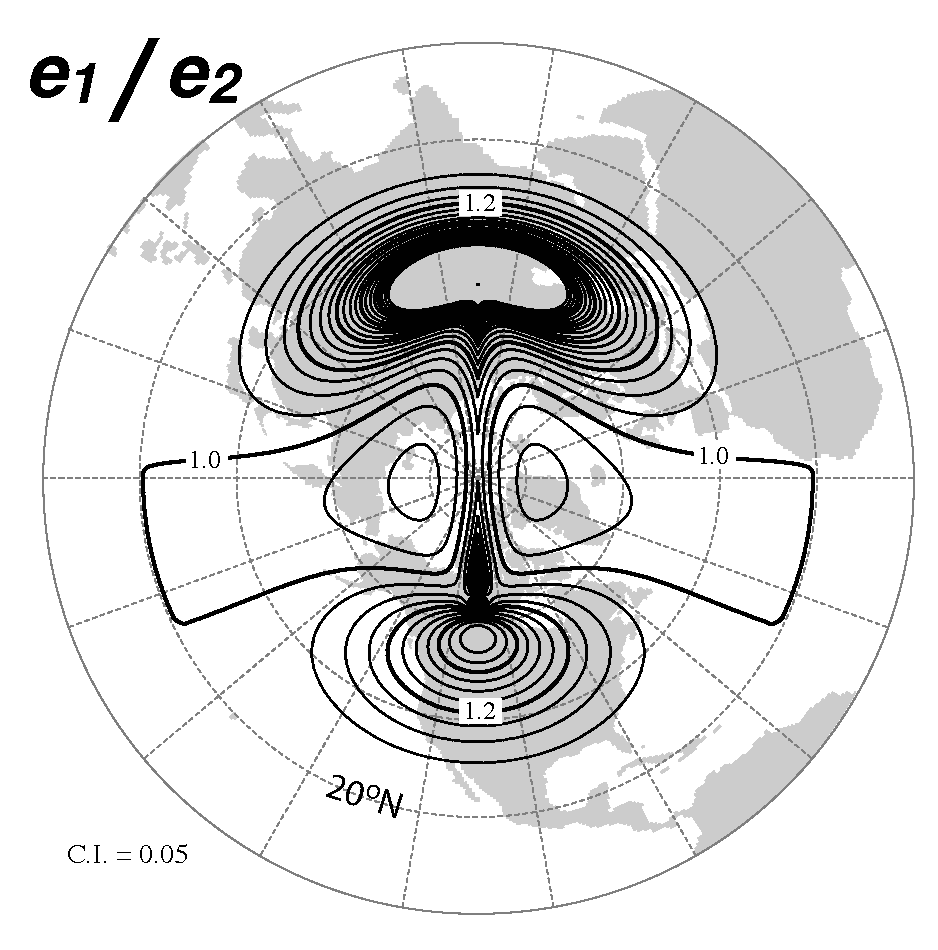
\includegraphics[width=0.66\textwidth]{CFGS_ORCA_aniso}
  \caption[Horizontal scale factors and ratio of anisotropy for ORCA 0.5\deg\ mesh]{
    \textit{Top}: Horizontal scale factors ($e_1$, $e_2$) and
    \textit{Bottom}: ratio of anisotropy ($e_1 / e_2$)
    for ORCA 0.5\deg\ mesh.
    South of 20\deg{N} a Mercator grid is used ($e_1 = e_2$) so that the anisotropy ratio is 1.
    Poleward of 20\deg{N},
    the two "north pole" introduce a weak anisotropy over the ocean areas ($< 1.2$) except in
    vicinity of Victoria Island (Canadian Arctic Archipelago).}
  \label{fig:CFGS_ORCA_e1e2}
\end{figure}

The method is applied to Mercator grid (\ie\ same zonal and meridional grid spacing) poleward of 20\deg{N},
so that the Equator is a mesh line, which provides a better numerical solution for equatorial dynamics.
The choice of the series of embedded ellipses (position of the foci and variation of the ellipses)
is a compromise between maintaining the ratio of mesh anisotropy ($e_1 / e_2$) close to one in the ocean
(especially in area of strong eddy activities such as the Gulf Stream) and keeping the smallest scale factor in
the northern hemisphere larger than the smallest one in the southern hemisphere.
The resulting mesh is shown in \autoref{fig:CFGS_ORCA_msh} and \autoref{fig:CFGS_ORCA_e1e2} for
a half a degree grid (ORCA\_R05).
The smallest ocean scale factor is found in along Antarctica,
while the ratio of anisotropy remains close to one except near the Victoria Island in the Canadian Archipelago.

%% =================================================================================================
\subsection{ORCA pre-defined resolution}
\label{subsec:CFGS_orca_resolution}

The \NEMO\ system is provided with five built-in ORCA configurations which differ in the horizontal resolution.
The value of the resolution is given by the resolution at the Equator expressed in degrees.
Each of configuration is set through the \textit{domain\_cfg} domain configuration file,
which sets the grid size and configuration name parameters.
The \NEMO\ System Team provides only ORCA2 domain input file "\textit{ORCA\_R2\_zps\_domcfg.nc}" file
(\autoref{tab:CFGS_ORCA}).

\begin{table}[!t]
  \centering
  \begin{tabular}{p{4cm} c c c c}
    Horizontal Grid & \texttt{ORCA\_index} & \texttt{jpiglo} & \texttt{jpjglo} \\
    \hline \hline
    % 4   \deg\ &              4   &          92 &          76 \\
    2   \deg\ &              2   &         182 &         149 \\
    1   \deg\ &              1   &         362 &         292 \\
    0.5 \deg\ &              05  &         722 &         511 \\
    0.25\deg\ &              025 &        1442 &        1021 \\
    \hline \hline
  \end{tabular}
  \caption[Domain size of ORCA family configurations]{
    Domain size of ORCA family configurations.
    The flag for configurations of ORCA family need to be set in \textit{domain\_cfg} file.}
  \label{tab:CFGS_ORCA}
\end{table}

The ORCA\_R2 configuration has the following specificity: starting from a 2\deg\ ORCA mesh,
local mesh refinements were applied to the Mediterranean, Red, Black and Caspian Seas,
so that the resolution is 1\deg\ there.
A local transformation were also applied with in the Tropics in order to refine the meridional resolution up to
0.5\deg\ at the Equator.

The ORCA\_R1 configuration has only a local tropical transformation to refine the meridional resolution up to
1/3\deg\ at the Equator.
Note that the tropical mesh refinements in ORCA\_R2 and R1 strongly increases the mesh anisotropy there.

The ORCA\_R05 and higher global configurations do not incorporate any regional refinements.

For ORCA\_R1 and R025, setting the configuration key to 75 allows to use 75 vertical levels, otherwise 46 are used.
In the other ORCA configurations, 31 levels are used
(see \autoref{tab:CFGS_ORCA}). %\sfcomment{HERE I need to put new table for ORCA2 values} and \autoref{fig:DOM_zgr_e3}).

Only the ORCA\_R2 is provided with all its input files in the \NEMO\ distribution.
%It is very similar to that used as part of the climate model developed at IPSL for the 4th IPCC assessment of
%climate change (Marti et al., 2009).
%It is also the basis for the \NEMO\ contribution to the Coordinate Ocean-ice Reference Experiments (COREs)
%documented in \citet{griffies.biastoch.ea_OM09}.

This version of ORCA\_R2 has 31 levels in the vertical, with the highest resolution (10m) in the upper 150m
(see \autoref{tab:CFGS_ORCA} and \autoref{fig:DOM_zgr_e3}).
The bottom topography and the coastlines are derived from the global atlas of Smith and Sandwell (1997).
The default forcing uses the boundary forcing from \citet{large.yeager_trpt04} (see \autoref{subsec:SBC_blk_ocean}),
which was developed for the purpose of running global coupled ocean-ice simulations without
an interactive atmosphere.
This \citet{large.yeager_trpt04} dataset is available through
the \href{http://nomads.gfdl.noaa.gov/nomads/forms/mom4/CORE.html}{GFDL web site}.
The "normal year" of \citet{large.yeager_trpt04} has been chosen of the \NEMO\ distribution since release v3.3.

ORCA\_R2 pre-defined configuration can also be run with multiply online nested zooms (\ie\ with AGRIF, \key{agrif} defined).
This is available as the AGRIF\_DEMO configuration that can be found in the \path{./cfgs/AGRIF_DEMO/} directory.

A regional Arctic or peri-Antarctic configuration is extracted from an ORCA\_R2 or R05 configurations using
sponge layers at open boundaries.

%% =================================================================================================
\section{GYRE family: double gyre basin}
\label{sec:CFGS_gyre}

The GYRE configuration \citep{levy.klein.ea_OM10} has been built to
simulate the seasonal cycle of a double-gyre box model.
It consists in an idealized domain similar to that used in the studies of \citet{drijfhout_JPO94} and
\citet{hazeleger.drijfhout_JPO98, hazeleger.drijfhout_JPO99, hazeleger.drijfhout_JGR00, hazeleger.drijfhout_JPO00},
over which an analytical seasonal forcing is applied.
This allows to investigate the spontaneous generation of a large number of interacting, transient mesoscale eddies
and their contribution to the large scale circulation.

The GYRE configuration run together with the PISCES biogeochemical model (GYRE-PISCES).
The domain geometry is a closed rectangular basin on the $\beta$-plane centred at $\sim$ 30\deg{N} and
rotated by 45\deg, 3180~km long, 2120~km wide and 4~km deep (\autoref{fig:MISC_strait_hand}).
The domain is bounded by vertical walls and by a flat bottom.
The configuration is meant to represent an idealized North Atlantic or North Pacific basin.
The circulation is forced by analytical profiles of wind and buoyancy fluxes.
The applied forcings vary seasonally in a sinusoidal manner between winter and summer extrema \citep{levy.klein.ea_OM10}.
The wind stress is zonal and its curl changes sign at 22\deg{N} and 36\deg{N}.
It forces a subpolar gyre in the north, a subtropical gyre in the wider part of the domain and
a small recirculation gyre in the southern corner.
The net heat flux takes the form of a restoring toward a zonal apparent air temperature profile.
A portion of the net heat flux which comes from the solar radiation is allowed to penetrate within the water column.
The fresh water flux is also prescribed and varies zonally.
It is determined such as, at each time step, the basin-integrated flux is zero.
The basin is initialised at rest with vertical profiles of temperature and salinity uniformly applied to
the whole domain.

The GYRE configuration is set like an analytical configuration by setting 
 \np[=.false.]{ln_read_cfg}{ln\_read\_cfg} in \nam{cfg}{cfg} part of the reference configuration
namelist \path{./cfgs/GYRE_PISCES/EXPREF/namelist_cfg}.
The analytical definition of grid in GYRE is done in \mdl{usrdef\_hrg} and \mdl{usrdef\_zgr} routines.
Its horizontal resolution (and thus the size of the domain) is determined by
setting \np{nn_GYRE}{nn\_GYRE} in \nam{usr_def}{usr\_def}:

\begin{align*}
   jpiglo = 30 \times \text{\np{nn_GYRE}{nn\_GYRE}} + 2 + 2 \times \text{\np{nn_hls}{nn\_hls}} \\
   jpjglo = 20 \times \text{\np{nn_GYRE}{nn\_GYRE}} + 2 + 2 \times \text{\np{nn_hls}{nn\_hls}}
\end{align*}

Obviously, the namelist parameters have to be adjusted to the chosen resolution,
see the Configurations pages on the \NEMO\ web site (\NEMO\ Configurations).
In the vertical, GYRE uses the default 30 ocean levels (\forcode{jpk = 31}, \autoref{fig:DOM_zgr_e3}).

\begin{listing}
  \begin{forlines}
!-----------------------------------------------------------------------
&namusr_def    !   GYRE user defined namelist  
!-----------------------------------------------------------------------
   nn_GYRE     =     1     !  GYRE resolution [1/degrees]
   ln_bench    = .false.   !  ! =T benchmark with gyre: the gridsize is kept constant
   jpkglo      =    31     !  number of model levels
/
  \end{forlines}
  \caption{\forcode{&namusr_def}}
  \label{lst:namusr_def}
\end{listing}

The GYRE configuration is also used in benchmark test as it is very simple to increase its resolution and
as it does not requires any input file.
For example, keeping a same model size on each processor while increasing the number of processor used is very easy,
even though the physical integrity of the solution can be compromised.
Benchmark is activate via \np[=.true.]{ln_bench}{ln\_bench} in \nam{usr_def}{usr\_def} in
namelist \path{./cfgs/GYRE_PISCES/EXPREF/namelist_cfg}.

\begin{figure}[!t]
  \centering
  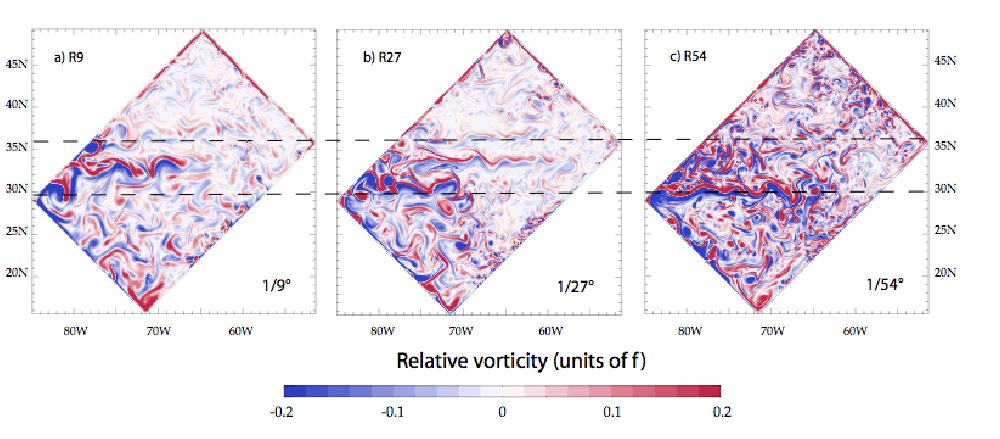
\includegraphics[width=0.66\textwidth]{CFGS_GYRE}
  \caption[Snapshot of relative vorticity at the surface of the model domain in GYRE R9, R27 and R54]{
    Snapshot of relative vorticity at the surface of the model domain in GYRE R9, R27 and R54.
    From \citet{levy.klein.ea_OM10}.}
  \label{fig:CFGS_GYRE}
\end{figure}

%% =================================================================================================
\section{AMM: atlantic margin configuration}
\label{sec:CFGS_config_AMM}

The AMM, Atlantic Margins Model, is a regional model covering the Northwest European Shelf domain on
a regular lat-lon grid at approximately 12km horizontal resolution.
The appropriate \textit{\&namcfg} namelist  is available in \path{./cfgs/AMM12/EXPREF/namelist\_cfg}.
It is used to build the correct dimensions of the AMM domain.

This configuration tests several features of \NEMO\ functionality specific to the shelf seas.
In particular, the AMM uses $s$-coordinates in the vertical rather than $z$-coordinates and
is forced with tidal lateral boundary conditions using a Flather boundary condition from the BDY module.
Also specific to the AMM configuration is the use of the GLS turbulence scheme (\np[=.true.]{ln_zdfgls}{ln\_zdfgls}).

In addition to the tidal boundary condition the model may also take open boundary conditions from
a North Atlantic model.
Boundaries may be completely omitted by setting \np{ln_bdy}{ln\_bdy} to false.
Sample surface fluxes, river forcing and a sample initial restart file are included to test a realistic model run.
The Baltic boundary is included within the river input file and is specified as a river source.
Unlike ordinary river points the Baltic inputs also include salinity and temperature data.

\subinc{%% =================================================================================================
%% Backmatter
%% =================================================================================================

%% Bibliography
%% =================================================================================================

\phantomsection
\addcontentsline{toc}{chapter}{Bibliography}
\lohead{Bibliography}
\rehead{Bibliography}
\bibliography{../main/bibliography}

\clearpage

%% Indices
%% =================================================================================================

\phantomsection
\addcontentsline{toc}{chapter}{Indices}
\lohead{Indices}
\rehead{Indices}
\printindex[blocks]
\printindex[keys]
\printindex[modules]
\printindex[parameters]
\printindex[subroutines]

\clearpage

%% Glossary
%% =================================================================================================

%\phantomsection
%\addcontentsline{toc}{chapter}{Glossary}
%\lohead{Glossary}\rehead{Glossary}
%\printglossaries
}

\end{document}
